\section{Diagnosis on RAG for Improvements}
\label{appendix:diagnosis}
% \begin{table}[h]
\caption{Overall metrics for RAG systems}
\centering
\resizebox{\textwidth}{!}{%
\begin{tabular}{lcccccccccccc}
\toprule
\multirow{2.5}{*}{Dataset} & 
\multirow{2.5}{*}{$k$} & 
\multicolumn{3}{c}{Overall} & 
\multicolumn{2}{c}{Retriever} & 
\multicolumn{6}{c}{Generator} \\
\cmidrule(lr){3-5} \cmidrule(lr){6-7} \cmidrule(lr){8-13}
 & & Prec.$\uparrow$ & Rec.$\uparrow$ & F1$\uparrow$ & CR$\uparrow$ & CP$\uparrow$ & CU$\uparrow$ & NS(I)$\downarrow$ & NS(II)$\downarrow$ & Hallu.$\downarrow$ & SK$\downarrow$ & Faith.$\uparrow$ \\
 \midrule
\rowcolor{Blue}
\multicolumn{13}{c}{\textbf{BM25 + GPT-4}} \\
\multirow{3}{*}{RobustQA-Finance}
 & 5 & 53.4 & 46.8 & 49.9 & 51.0 & 60.8 & 68.7 & 21.8 & 4.8 & 20.0 & 9.7 & 70.2 \\
 & 10 & 54.8 & 48.9 & 51.7 & 60.9 & 56.6 & 65.4 & 23.6 & 4.2 & 17.3 & 6.9 & 75.7 \\
 & 20 & 54.0 & 50.1 & 52.0 & 69.4 & 52.1 & 62.3 & 26.8 & 3.9 & 15.4 & 4.7 & 79.9 \\
\multirow{3}{*}{RobustQA-Writing}
 & 5 & 76.0 & 62.5 & 68.6 & 72.6 & 78.2 & 74.5 & 16.0 & 1.3 & 6.7 & 8.1 & 85.2 \\
 & 10 & 75.6 & 63.5 & 69.0 & 81.0 & 72.4 & 72.0 & 17.5 & 1.3 & 5.6 & 5.2 & 89.2 \\
 & 20 & 76.4 & 63.6 & 69.4 & 86.3 & 64.3 & 70.0 & 17.5 & 1.0 & 5.1 & 4.0 & 90.9 \\
\multirow{3}{*}{KIWI}
 & 5 & 42.6 & 28.9 & 34.4 & 36.6 & 78.9 & 66.3 & 41.3 & 7.2 & 8.9 & 3.7 & 87.3 \\
 & 10 & 42.2 & 29.1 & 34.5 & 45.6 & 74.9 & 58.0 & 43.8 & 7.1 & 6.9 & 2.1 & 91.1 \\
 & 20 & 42.8 & 30.0 & 35.3 & 57.8 & 72.5 & 49.1 & 45.0 & 6.2 & 6.0 & 0.7 & 93.3 \\
\rowcolor{Blue}
\multicolumn{13}{c}{\textbf{E5-Mistral + GPT-4}} \\
\multirow{3}{*}{RobustQA-Finance}
 & 5 & 57.6 & 54.0 & 55.8 & 71.5 & 77.8 & 69.0 & 27.5 & 3.0 & 12.0 & 3.4 & 84.7 \\
 & 10 & 57.0 & 55.0 & 56.0 & 80.1 & 72.6 & 64.3 & 29.5 & 2.8 & 10.7 & 2.4 & 86.9 \\
 & 20 & 56.1 & 54.6 & 55.3 & 86.3 & 67.4 & 60.2 & 31.7 & 2.7 & 9.5 & 1.4 & 89.1 \\
\multirow{3}{*}{RobustQA-Writing}
 & 5 & 77.7 & 65.6 & 71.1 & 81.6 & 81.4 & 75.6 & 15.7 & 1.5 & 5.1 & 3.3 & 91.6 \\
 & 10 & 77.6 & 66.1 & 71.4 & 88.1 & 74.7 & 72.7 & 16.9 & 1.7 & 3.7 & 1.8 & 94.4 \\
 & 20 & 77.1 & 65 & 70.5 & 91.7 & 66.3 & 69 & 17.9 & 1.2 & 3.8 & 1.3 & 94.9 \\
\multirow{3}{*}{KIWI}
 & 5 & 43.5 & 29.9 & 35.4 & 43.5 & 91.0 & 58.6 & 44.9 & 2.8 & 8.7 & 2.0 & 89.2 \\
 & 10 & 44.9 & 31.8 & 37.3 & 52.9 & 88.9 & 53.4 & 44.5 & 3.1 & 7.5 & 2.2 & 90.3 \\
 & 20 & 45.5 & 34.0 & 38.9 & 64.6 & 86.7 & 49.0 & 44.9 & 4.0 & 5.5 & 1.5 & 93.0 \\
\rowcolor{Blue}
\multicolumn{13}{c}{\textbf{E5-Mistral + Llama3 70B}} \\
\multirow{3}{*}{RobustQA-Finance}
 & 5 & 57.3 & 49.0 & 52.8 & 71.6 & 77.9 & 64.2 & 34.2 & 3.9 & 4.7 & 1.9 & 93.4 \\
 & 10 & 55.7 & 51.7 & 53.6 & 80.0 & 72.5 & 61.2 & 35.5 & 4.7 & 4.1 & 1.0 & 94.9 \\
 & 20 & 56.0 & 51.4 & 53.6 & 86.3 & 67.4 & 57.5 & 35.2 & 3.9 & 4.9 & 0.6 & 94.4 \\
\multirow{3}{*}{RobustQA-Writing}
 & 5 & 72.1 & 61.3 & 66.2 & 81.6 & 81.4 & 71.7 & 23.2 & 2.1 & 2.5 & 1.1 & 96.3 \\
 & 10 & 74.2 & 65.6 & 69.6 & 88.1 & 74.7 & 72.3 & 22.3 & 1.8 & 1.7 & 1.1 & 97.1 \\
 & 20 & 73.1 & 65.7 & 69.2 & 91.7 & 66.3 & 70.1 & 23.5 & 1.9 & 1.5 & 0.5 & 98.0 \\
\multirow{3}{*}{KIWI}
 & 5 & 40.5 & 25.1 & 31.0 & 43.5 & 91.0 & 48.3 & 51.1 & 3.9 & 4.6 & 0.7 & 94.7 \\
 & 10 & 41.8 & 28.1 & 33.6 & 52.9 & 88.9 & 48.9 & 51.8 & 3.7 & 2.6 & 0.4 & 97.0 \\
 & 20 & 45.2 & 30.9 & 36.7 & 64.6 & 86.7 & 45.3 & 47.5 & 3.7 & 3.6 & 0.3 & 96.1 \\
\bottomrule
\end{tabular}
}
\end{table}
% \begin{table}[h]
\caption{Overall metrics for RAG systems}
\centering
\resizebox{\textwidth}{!}{%
\begin{tabular}{lcccccccccccc}
\toprule
\multirow{2.5}{*}{Dataset} & 
\multirow{2.5}{*}{Prompt} & 
\multicolumn{3}{c}{Overall metrics} & 
\multicolumn{2}{c}{Retriever metrics} & 
\multicolumn{6}{c}{Generator metrics} \\
\cmidrule(lr){3-5} \cmidrule(lr){6-7} \cmidrule(lr){8-13} 
 &  & Prec.$\uparrow$ & Rec.$\uparrow$ & F1$\uparrow$ & CR$\uparrow$ & CP$\uparrow$ & CU$\uparrow$ & NS(I)$\downarrow$ & NS(II)$\downarrow$ & Hallu.$\downarrow$ & SK$\downarrow$ & Faith.$\uparrow$ \\
\midrule
\rowcolor{Blue} 
\multicolumn{13}{c}{\textbf{BM25 + GPT-4}} \\
\multirow{2}{*}{RobustQA-Finance} & basic & 54.0 & 50.1 & 52.0 & 69.4 & 52.1 & 62.3 & 26.8 & 3.9 & 15.4 & 4.7 & 79.9 \\
 & optim. & 53.1 & 52.4 & 52.7 & 69.4 & 52.1 & 66.2 & 31.0 & 5.1 & 10.7 & 3.3 & 86.0 \\
\multirow{2}{*}{RobustQA-Writing} & basic & 76.4 & 63.6 & 69.4 & 86.3 & 64.3 & 70.0 & 17.5 & 1.0 & 5.1 & 4.0 & 90.9 \\
 & optim. & 75.0 & 66.6 & 70.6 & 86.3 & 64.3 & 73.0 & 19.3 & 2.1 & 3.6 & 3.6 & 92.9 \\
\multirow{2}{*}{KIWI} & basic & 42.8 & 30.0 & 35.3 & 57.8 & 72.5 & 49.1 & 45.0 & 6.2 & 6.0 & 0.7 & 93.3 \\
 & optim. & 41.0 & 34.6 & 37.6 & 57.8 & 72.5 & 57.0 & 48.6 & 4.5 & 5.8 & 1.4 & 92.8 \\
\rowcolor{Blue} 
\multicolumn{13}{c}{\textbf{E5-Mistral + GPT-4}} \\
\multirow{2}{*}{RobustQA-Finance} & basic & 56.1 & 54.6 & 55.3 & 86.3 & 67.4 & 60.2 & 31.7 & 2.7 & 9.5 & 1.4 & 89.1 \\
 & optim. & 54.4 & 60.7 & 57.4 & 86.3 & 67.4 & 67.1 & 35.5 & 3.4 & 6.8 & 1.5 & 91.7 \\
\multirow{2}{*}{RobustQA-Writing} & basic & 77.1 & 65.0 & 70.5 & 91.7 & 66.3 & 69.0 & 17.9 & 1.2 & 3.8 & 1.3 & 94.9 \\
 & optim. & 76.7 & 69.2 & 72.8 & 91.7 & 66.3 & 73.6 & 19.6 & 1.2 & 2.5 & 0.9 & 96.6 \\
\multirow{2}{*}{KIWI} & basic & 45.5 & 34.0 & 38.9 & 64.6 & 86.7 & 49.0 & 44.9 & 4.0 & 5.5 & 1.5 & 93.0 \\
 & optim. & 44.5 & 38.1 & 41.0 & 64.6 & 86.7 & 53.8 & 48.0 & 3.3 & 4.2 & 1.0 & 94.8 \\
\rowcolor{Blue}
\multicolumn{13}{c}{\textbf{E5-Mistral + Llama3 70B}} \\
\multirow{2}{*}{RobustQA-Finance} & basic & 56.0 & 51.4 & 53.6 & 86.3 & 67.4 & 57.5 & 35.2 & 3.9 & 4.9 & 0.6 & 94.4 \\
 & optim. & 53.7 & 55.2 & 54.5 & 86.3 & 67.4 & 61.5 & 37.5 & 3.8 & 5.0 & 1.0 & 94.0 \\
\multirow{2}{*}{RobustQA-Writing} & basic & 73.1 & 65.7 & 69.2 & 91.7 & 66.3 & 70.1 & 23.5 & 1.9 & 1.5 & 0.5 & 98.0 \\
 & optim. & 70.8 & 68.9 & 69.8 & 91.7 & 66.3 & 73.6 & 25.4 & 1.7 & 2.1 & 0.4 & 97.4 \\
\multirow{2}{*}{KIWI} & basic & 45.2 & 30.9 & 36.7 & 64.7 & 86.9 & 45.3 & 47.5 & 3.7 & 3.6 & 0.3 & 96.1 \\
 & optim. & 43.8 & 31.6 & 36.7 & 64.7 & 86.9 & 47.4 & 49.5 & 3.1 & 3.5 & 0.2 & 96.3 \\
\bottomrule
\end{tabular}
}
\end{table}
% \begin{table}[h]
\caption{Overall metrics for RAG systems by dataset and model}
\centering
\resizebox{\textwidth}{!}{
\begin{tabular}{lcccccccccccc}
\toprule
\multirow{2.5}{*}{Dataset} & 
\multirow{2.5}{*}{Chunk Size} & 
\multicolumn{3}{c}{Overall} & 
\multicolumn{2}{c}{Retriever} & 
\multicolumn{6}{c}{Generator}\\
\cmidrule(lr){3-5} \cmidrule(lr){6-7} \cmidrule(lr){8-13} 
 & & Prec.$\uparrow$ & Rec.$\uparrow$ & F1$\uparrow$ & CR$\uparrow$ & CP$\uparrow$ & CU$\uparrow$ & NS(I)$\downarrow$ & NS(II)$\downarrow$ & Hallu.$\downarrow$ & SK$\downarrow$ & Faith.$\uparrow$ \\
\midrule
\rowcolor{Blue}
\multicolumn{13}{c}{\textbf{BM25 + GPT-4}} \\
\multirow{4}{*}{RobustQA-Finance} & 100 & 53.7 & 44.7 & 48.8 & 53.8 & 43.5 & 65.9 & 21.8 & 6.7 & 17.8 & 7.8 & 74.4 \\
 & 150 & 54.8 & 47.0 & 50.6 & 61.4 & 47.2 & 65.2 & 23.6 & 5.5 & 16.1 & 6.3 & 77.6 \\
 & 300 & 54.0 & 50.1 & 52.0 & 69.4 & 52.1 & 62.3 & 26.8 & 3.9 & 15.4 & 4.7 & 79.9 \\
 & 600 & 54.9 & 50.5 & 52.6 & 73.4 & 53.8 & 61.7 & 28.7 & 3.5 & 12.9 & 3.9 & 83.2 \\
\multirow{4}{*}{RobustQA-Writing} & 100 & 75.7 & 60.9 & 67.5 & 76.9 & 58.5 & 72.2 & 16.1 & 2.1 & 6.2 & 4.8 & 89.1 \\
 & 150 & 75.0 & 62.4 & 68.1 & 82.1 & 61.3 & 70.1 & 17.7 & 1.6 & 5.6 & 4.2 & 90.2 \\
 & 300 & 76.4 & 63.6 & 69.4 & 86.3 & 64.3 & 70.0 & 17.5 & 1.0 & 5.1 & 4.0 & 90.9 \\
 & 600 & 75.9 & 64.4 & 69.6 & 87.8 & 63.6 & 69.3 & 17.9 & 1.3 & 5.0 & 3.2 & 91.8 \\
\multirow{4}{*}{KIWI} & 100 & 45.7 & 27.7 & 34.5 & 42.4 & 60.6 & 56.4 & 36.9 & 8.5 & 8.9 & 3.4 & 87.7 \\
 & 150 & 48.4 & 29.9 & 37.0 & 47.6 & 65.1 & 54.8 & 37.5 & 5.9 & 8.1 & 2.5 & 89.3 \\
 & 300 & 42.8 & 30.0 & 35.3 & 57.8 & 72.5 & 49.1 & 45.0 & 6.2 & 6.0 & 0.7 & 93.3 \\
 & 600 & 42.6 & 32.8 & 37.1 & 67.3 & 77.8 & 46.9 & 48.6 & 3.3 & 5.6 & 0.8 & 93.6 \\
\rowcolor{Blue}
\multicolumn{13}{c}{\textbf{E5-Mistral + GPT-4}} \\
\multirow{4}{*}{RobustQA-Finance} & 100 & 55.7 & 50.8 & 53.2 & 74.0 & 62.4 & 64.0 & 29.3 & 4.8 & 10.2 & 2.6 & 87.3 \\
 & 150 & 56.3 & 53.4 & 54.8 & 79.7 & 64.5 & 62.6 & 30.4 & 4.3 & 9.1 & 2.0 & 88.9 \\
 & 300 & 56.1 & 54.6 & 55.3 & 86.3 & 67.4 & 60.2 & 31.7 & 2.7 & 9.5 & 1.4 & 89.1 \\
 & 600 & 55.5 & 55.3 & 55.4 & 88.6 & 68.5 & 60.5 & 34.0 & 2.5 & 8.0 & 1.1 & 90.9 \\
\multirow{4}{*}{RobustQA-Writing} & 100 & 76.6 & 63.8 & 69.6 & 86.6 & 66.6 & 70.6 & 17.9 & 1.2 & 4.4 & 1.6 & 94.0 \\
 & 150 & 77.5 & 65.3 & 70.9 & 88.4 & 66.1 & 71.2 & 18.3 & 1.3 & 2.9 & 1.1 & 96.0 \\
 & 300 & 77.1 & 65.0 & 70.5 & 91.7 & 66.3 & 69.0 & 17.9 & 1.2 & 3.8 & 1.3 & 94.9 \\
 & 600 & 77.8 & 66.2 & 71.5 & 93.6 & 67.5 & 69.4 & 18.4 & 1.1 & 2.7 & 0.9 & 96.4 \\
\multirow{4}{*}{KIWI} & 100 & 46.9 & 28.5 & 35.4 & 51.3 & 80.6 & 49.8 & 41.7 & 4.4 & 7.0 & 2.5 & 90.5 \\
 & 150 & 46.6 & 29.6 & 36.2 & 52.6 & 79.6 & 51.1 & 42.0 & 3.8 & 7.6 & 1.8 & 90.5 \\
 & 300 & 45.5 & 34.0 & 38.9 & 64.6 & 86.7 & 49.0 & 44.9 & 4.0 & 5.5 & 1.5 & 93.0 \\
 & 600 & 47.0 & 34.5 & 39.8 & 75.8 & 90.7 & 43.4 & 47.0 & 0.8 & 5.2 & 0.8 & 94.0 \\
\rowcolor{Blue}
\multicolumn{13}{c}{\textbf{E5-Mistral + Llama3 70B}} \\
\multirow{4}{*}{RobustQA-Finance} & 100 & 53.8 & 47.4 & 50.4 & 74.0 & 62.4 & 60.5 & 34.3 & 7.2 & 4.6 & 1.4 & 94.0 \\
 & 150 & 55.7 & 50.9 & 53.2 & 79.7 & 64.5 & 60.2 & 34.2 & 6.1 & 3.9 & 0.8 & 95.3 \\
 & 300 & 56.0 & 51.4 & 53.6 & 86.3 & 67.4 & 57.5 & 35.2 & 3.9 & 4.9 & 0.6 & 94.4 \\
 & 600 & - & - & - & - & - & - & - & - & - & - & - \\
\multirow{4}{*}{RobustQA-Writing} & 100 & 71.7 & 61.7 & 66.3 & 86.6 & 66.6 & 69.1 & 24.4 & 1.5 & 2.4 & 1.0 & 96.6 \\
 & 150 & 72.2 & 63.9 & 67.8 & 88.4 & 66.1 & 70.1 & 23.9 & 1.8 & 2.1 & 0.3 & 97.6 \\
 & 300 & 73.1 & 65.7 & 69.2 & 91.7 & 66.3 & 70.1 & 23.5 & 1.9 & 1.5 & 0.5 & 98.0 \\
 & 600 & - & - & - & - & - & - & - & - & - & - & - \\
\multirow{4}{*}{KIWI} & 100 & 40.5 & 24.6 & 30.6 & 51.3 & 80.6 & 45.1 & 51.1 & 4.9 & 3.5 & 0.2 & 96.2 \\
 & 150 & 43.7 & 29.3 & 35.1 & 52.6 & 79.6 & 51.6 & 47.1 & 5.4 & 3.7 & 1.0 & 95.3 \\
 & 300 & 45.2 & 30.9 & 36.7 & 64.7 & 86.9 & 45.3 & 47.5 & 3.7 & 3.6 & 0.3 & 96.1 \\
 & 600 & - & - & - & - & - & - & - & - & - & - & - \\
\bottomrule
\end{tabular}
}
\end{table}
% \begin{table}[h]
\caption{Overall metrics for RAG systems with different chunk overlap ratios}
\centering
\resizebox{\textwidth}{!}{%
\begin{tabular}{lcccccccccccc}
\toprule
\multirow{2.5}{*}{Dataset} & 
\multirow{2.5}{*}{Overlap} & 
\multicolumn{3}{c}{Overall} & 
\multicolumn{2}{c}{Retriever} & 
\multicolumn{6}{c}{Generator} \\
\cmidrule(lr){3-5} \cmidrule(lr){6-7} \cmidrule(lr){8-13} 
 & & Prec.$\uparrow$ & Rec.$\uparrow$ & F1$\uparrow$ & CR$\uparrow$ & CP$\uparrow$ & CU$\uparrow$ & NS(I)$\downarrow$ & NS(II)$\downarrow$ & Hallu.$\downarrow$ & SK$\downarrow$ & Faith.$\uparrow$ \\
\midrule
\rowcolor{Blue}
\multicolumn{13}{c}{\textbf{BM25 + GPT-4}} \\
\multirow{3}{*}{RobustQA-Finance} & 0.0 & 53.9 & 50.1 & 51.9 & 69.4 & 51.6 & 63.1 & 27.2 & 4.3 & 14.6 & 4.1 & 81.2 \\
 & 0.2 & 54.0 & 50.1 & 52.0 & 69.4 & 52.1 & 62.3 & 26.8 & 3.9 & 15.4 & 4.7 & 79.9 \\
 & 0.4 & 53.3 & 50.4 & 51.8 & 70.0 & 53.1 & 62.9 & 27.7 & 3.8 & 15.2 & 4.2 & 80.6 \\
\multirow{3}{*}{RobustQA-Writing} & 0.0 & 76.5 & 63.7 & 69.5 & 86.5 & 63.1 & 69.8 & 17.8 & 1.0 & 4.6 & 4.0 & 91.4 \\
 & 0.2 & 76.4 & 63.6 & 69.4 & 86.3 & 64.3 & 70.0 & 17.5 & 1.0 & 5.1 & 4.0 & 90.9 \\
 & 0.4 & 76.0 & 64.9 & 70.0 & 86.4 & 65.5 & 71.4 & 18.0 & 1.1 & 4.9 & 3.3 & 91.8 \\
\multirow{3}{*}{KIWI} & 0.0 & 43.6 & 31.3 & 36.4 & 58.1 & 71.2 & 50.9 & 44.5 & 4.5 & 7.5 & 1.0 & 91.6 \\
 & 0.2 & 42.8 & 30.0 & 35.3 & 57.8 & 72.5 & 49.1 & 45.0 & 6.2 & 6.0 & 0.7 & 93.3 \\
 & 0.4 & 44.0 & 31.9 & 37.0 & 58.7 & 74.9 & 51.7 & 45.1 & 4.8 & 6.1 & 0.5 & 93.4 \\
\rowcolor{Blue}
\multicolumn{13}{c}{\textbf{E5-Mistral + GPT-4}} \\
\multirow{3}{*}{RobustQA-Finance} & 0.0 & 56.7 & 55.6 & 56.1 & 86.2 & 67.0 & 62.1 & 31.4 & 2.9 & 9.0 & 1.3 & 89.7 \\
& 0.2 & 56.1 & 54.6 & 55.3 & 86.3 & 67.4 & 60.2 & 31.7 & 2.7 & 9.5 & 1.4 & 89.1 \\
& 0.4 & 56.5 & 56.3 & 56.4 & 86.8 & 69.0 & 62.5 & 31.9 & 2.7 & 8.8 & 1.5 & 89.6 \\
\multirow{3}{*}{RobustQA-Writing} & 0.0 & 76.6 & 66.3 & 71.1 & 91.9 & 66.4 & 70.4 & 18.8 & 1.3 & 3.3 & 0.9 & 95.8 \\
& 0.2 & 77.1 & 65.0 & 70.5 & 91.7 & 66.3 & 69.0 & 17.9 & 1.2 & 3.8 & 1.3 & 94.9 \\
& 0.4 & 77.9 & 66.5 & 71.8 & 91.9 & 66.9 & 70.3 & 18.0 & 1.2 & 2.9 & 1.0 & 96.1 \\
\multirow{3}{*}{KIWI} & 0.0 & 47.4 & 33.8 & 39.5 & 65.1 & 85.7 & 46.6 & 44.2 & 2.4 & 6.0 & 1.0 & 93.0 \\
& 0.2 & 45.5 & 34.0 & 38.9 & 64.6 & 86.7 & 49.0 & 44.9 & 4.0 & 5.5 & 1.5 & 93.0 \\
& 0.4 & 46.1 & 32.7 & 38.2 & 65.1 & 87.1 & 46.3 & 45.2 & 2.9 & 5.8 & 0.8 & 93.3 \\
\rowcolor{Blue}
\multicolumn{13}{c}{\textbf{E5-Mistral + Llama3 70B}} \\
\multirow{3}{*}{RobustQA-Finance} & 0.0 & 56.9 & 53.6 & 55.2 & 86.2 & 67.0 & 59.7 & 34.6 & 3.5 & 5.0 & 0.6 & 94.4 \\
& 0.2 & 56.0 & 51.4 & 53.6 & 86.3 & 67.4 & 57.5 & 35.2 & 3.9 & 4.9 & 0.6 & 94.4 \\
& 0.4 & 56.8 & 52.7 & 54.7 & 86.8 & 69.0 & 58.4 & 35.6 & 3.7 & 3.9 & 0.8 & 95.3 \\
\multirow{3}{*}{RobustQA-Writing} & 0.0 & 72.4 & 66.0 & 69.1 & 91.9 & 66.4 & 70.5 & 23.5 & 1.8 & 2.3 & 0.4 & 97.3 \\
& 0.2 & 73.1 & 65.7 & 69.2 & 91.7 & 66.3 & 70.1 & 23.5 & 1.9 & 1.5 & 0.5 & 98.0 \\
& 0.4 & 72.4 & 65.7 & 68.9 & 91.9 & 66.9 & 70.0 & 23.8 & 1.6 & 2.3 & 0.5 & 97.2 \\
\multirow{3}{*}{KIWI} & 0.0 & 43.8 & 31.6 & 36.8 & 65.1 & 85.7 & 44.7 & 48.2 & 5.5 & 2.5 & 0.6 & 96.9 \\
& 0.2 & 45.2 & 30.9 & 36.7 & 64.7 & 86.9 & 45.3 & 47.5 & 3.7 & 3.6 & 0.3 & 96.1 \\
& 0.4 & 44.9 & 29.5 & 35.6 & 65.1 & 87.1 & 42.8 & 46.5 & 4.2 & 4.5 & 0.3 & 95.2 \\
\bottomrule
\end{tabular}
}
\end{table}


We modify hyper-parameters commonly tuned in RAG systems to observe performance variance under the metrics defined by \benchname\space. We focus on how \benchname\space explains this variance and provides tuning suggestions for improvements on certain aspects. In this section, we evaluate three RAG baselines (BM25\_GPT-4, E5-Mistral\_GPT-4, and E5-Mistral\_Llama3-70B) across three domains with increasing difficulty: Writing, Finance, and KIWI.
We use our default settings (Appendix~\ref{appendix:experiment_setup_detail}) in main experiments as controls.
We experiment with different numbers of chunks selected as context $k\in$\{5,10,20\}, different chunk size \{150,300,600\}\footnote{We omit chunk size of 600 for E5-Mistral\_Llama3-70B due to the limited 8K context window of Llama3.}, different chunk overlap ratio \{0.0,0.2,0.4\}, and different generation prompts.

\begin{figure}[ht]
    \centering
    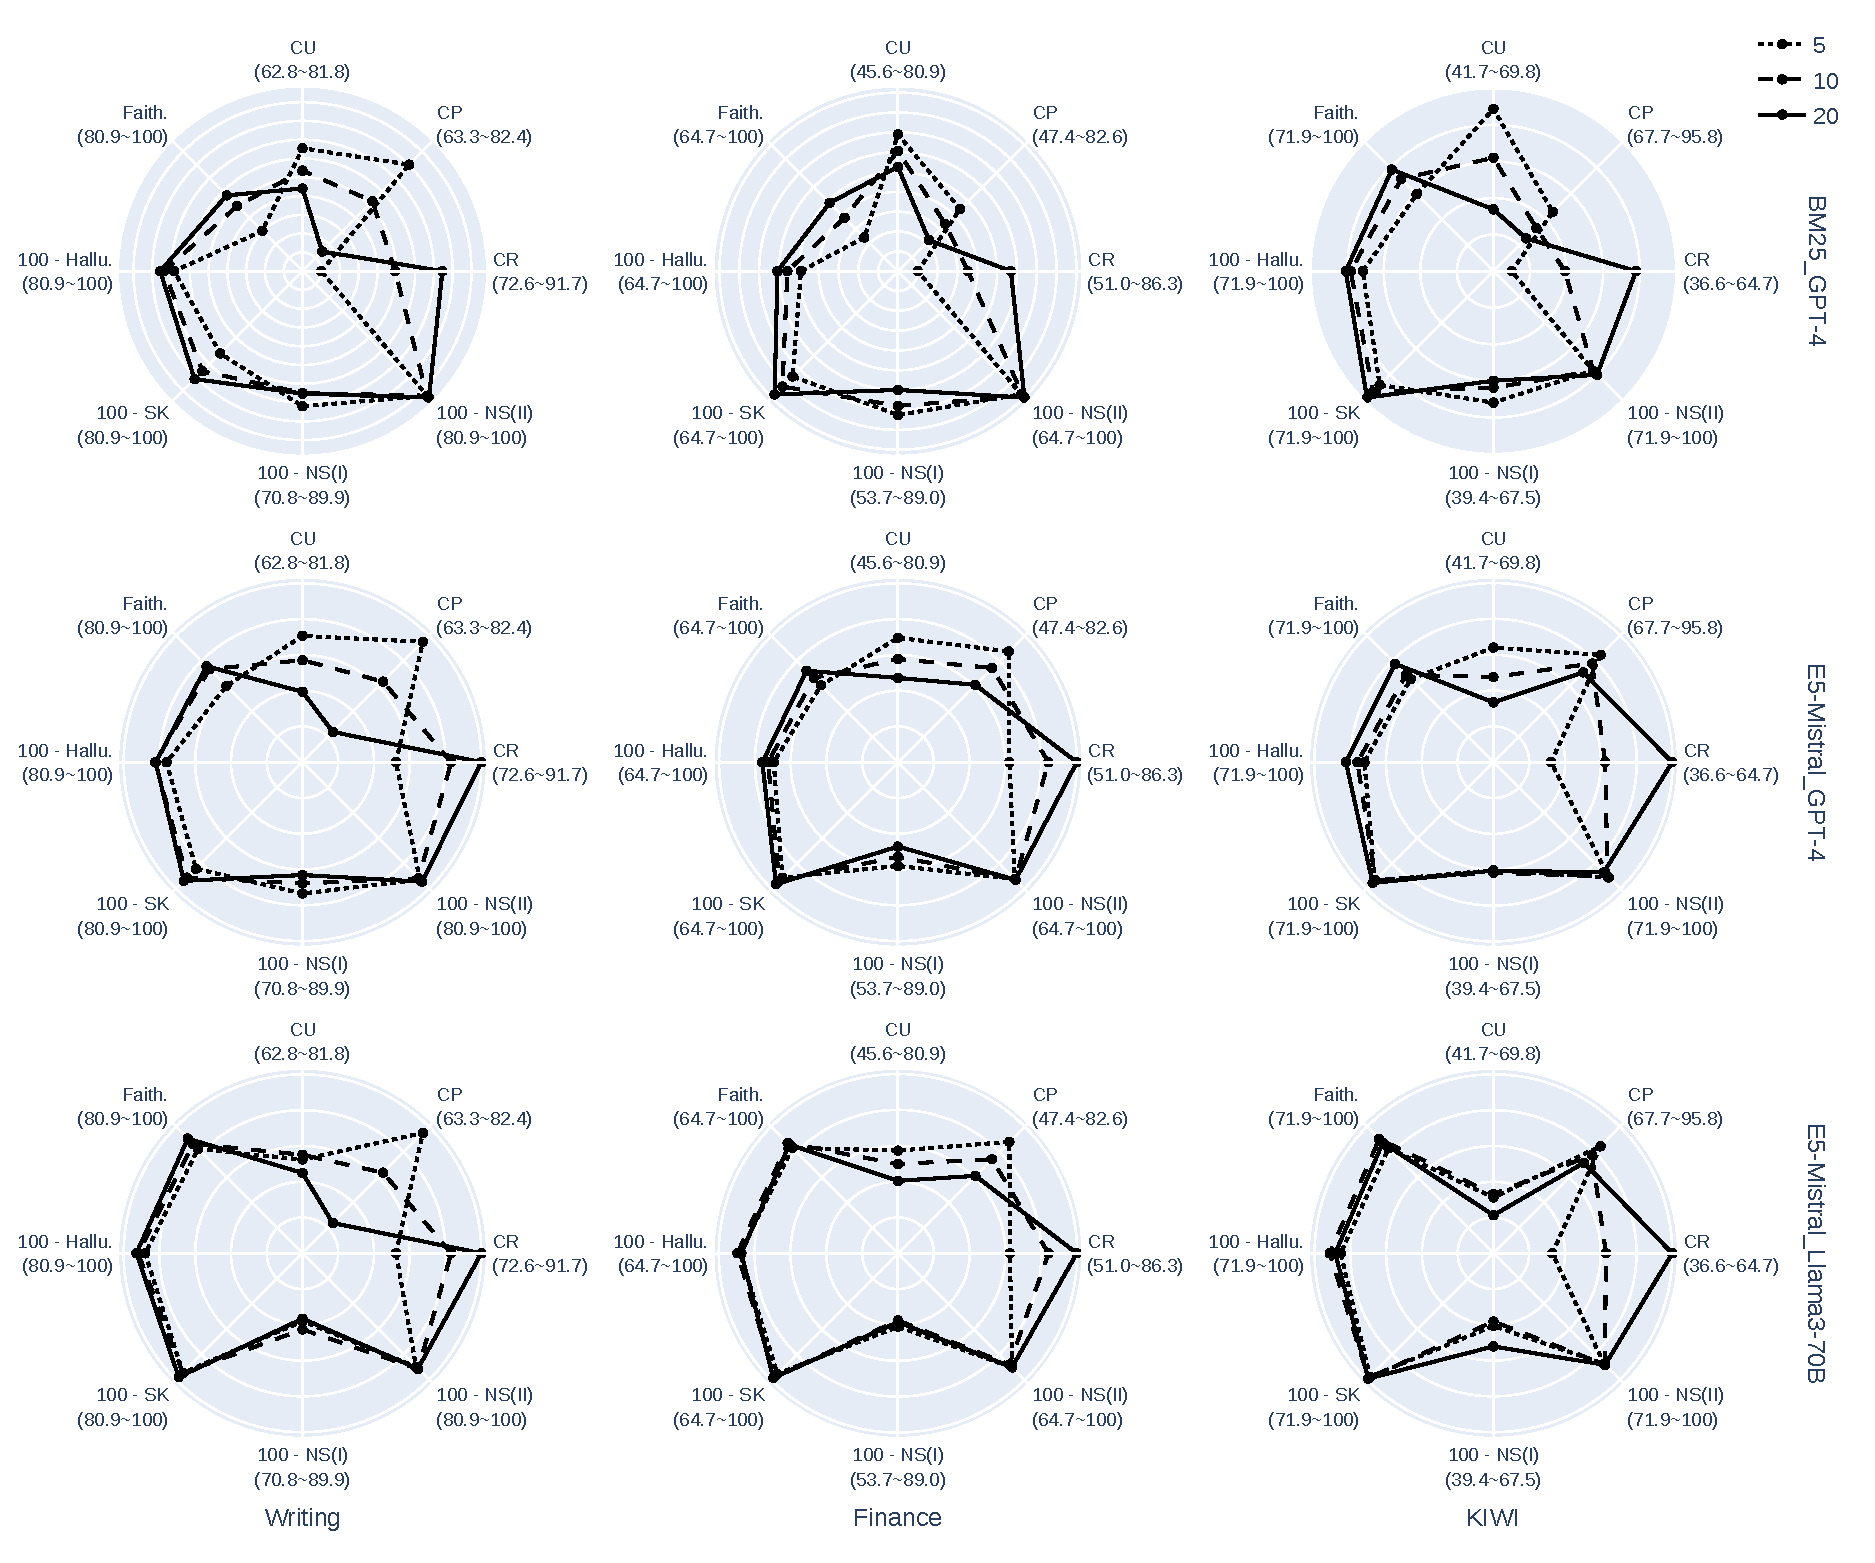
\includegraphics[width=\columnwidth]{figures/radar_topk.pdf}
    \caption{Diagnosis on Top-k Selection}
    \label{fig:radar-topk}
\end{figure}

\begin{figure}[ht]
    \centering
    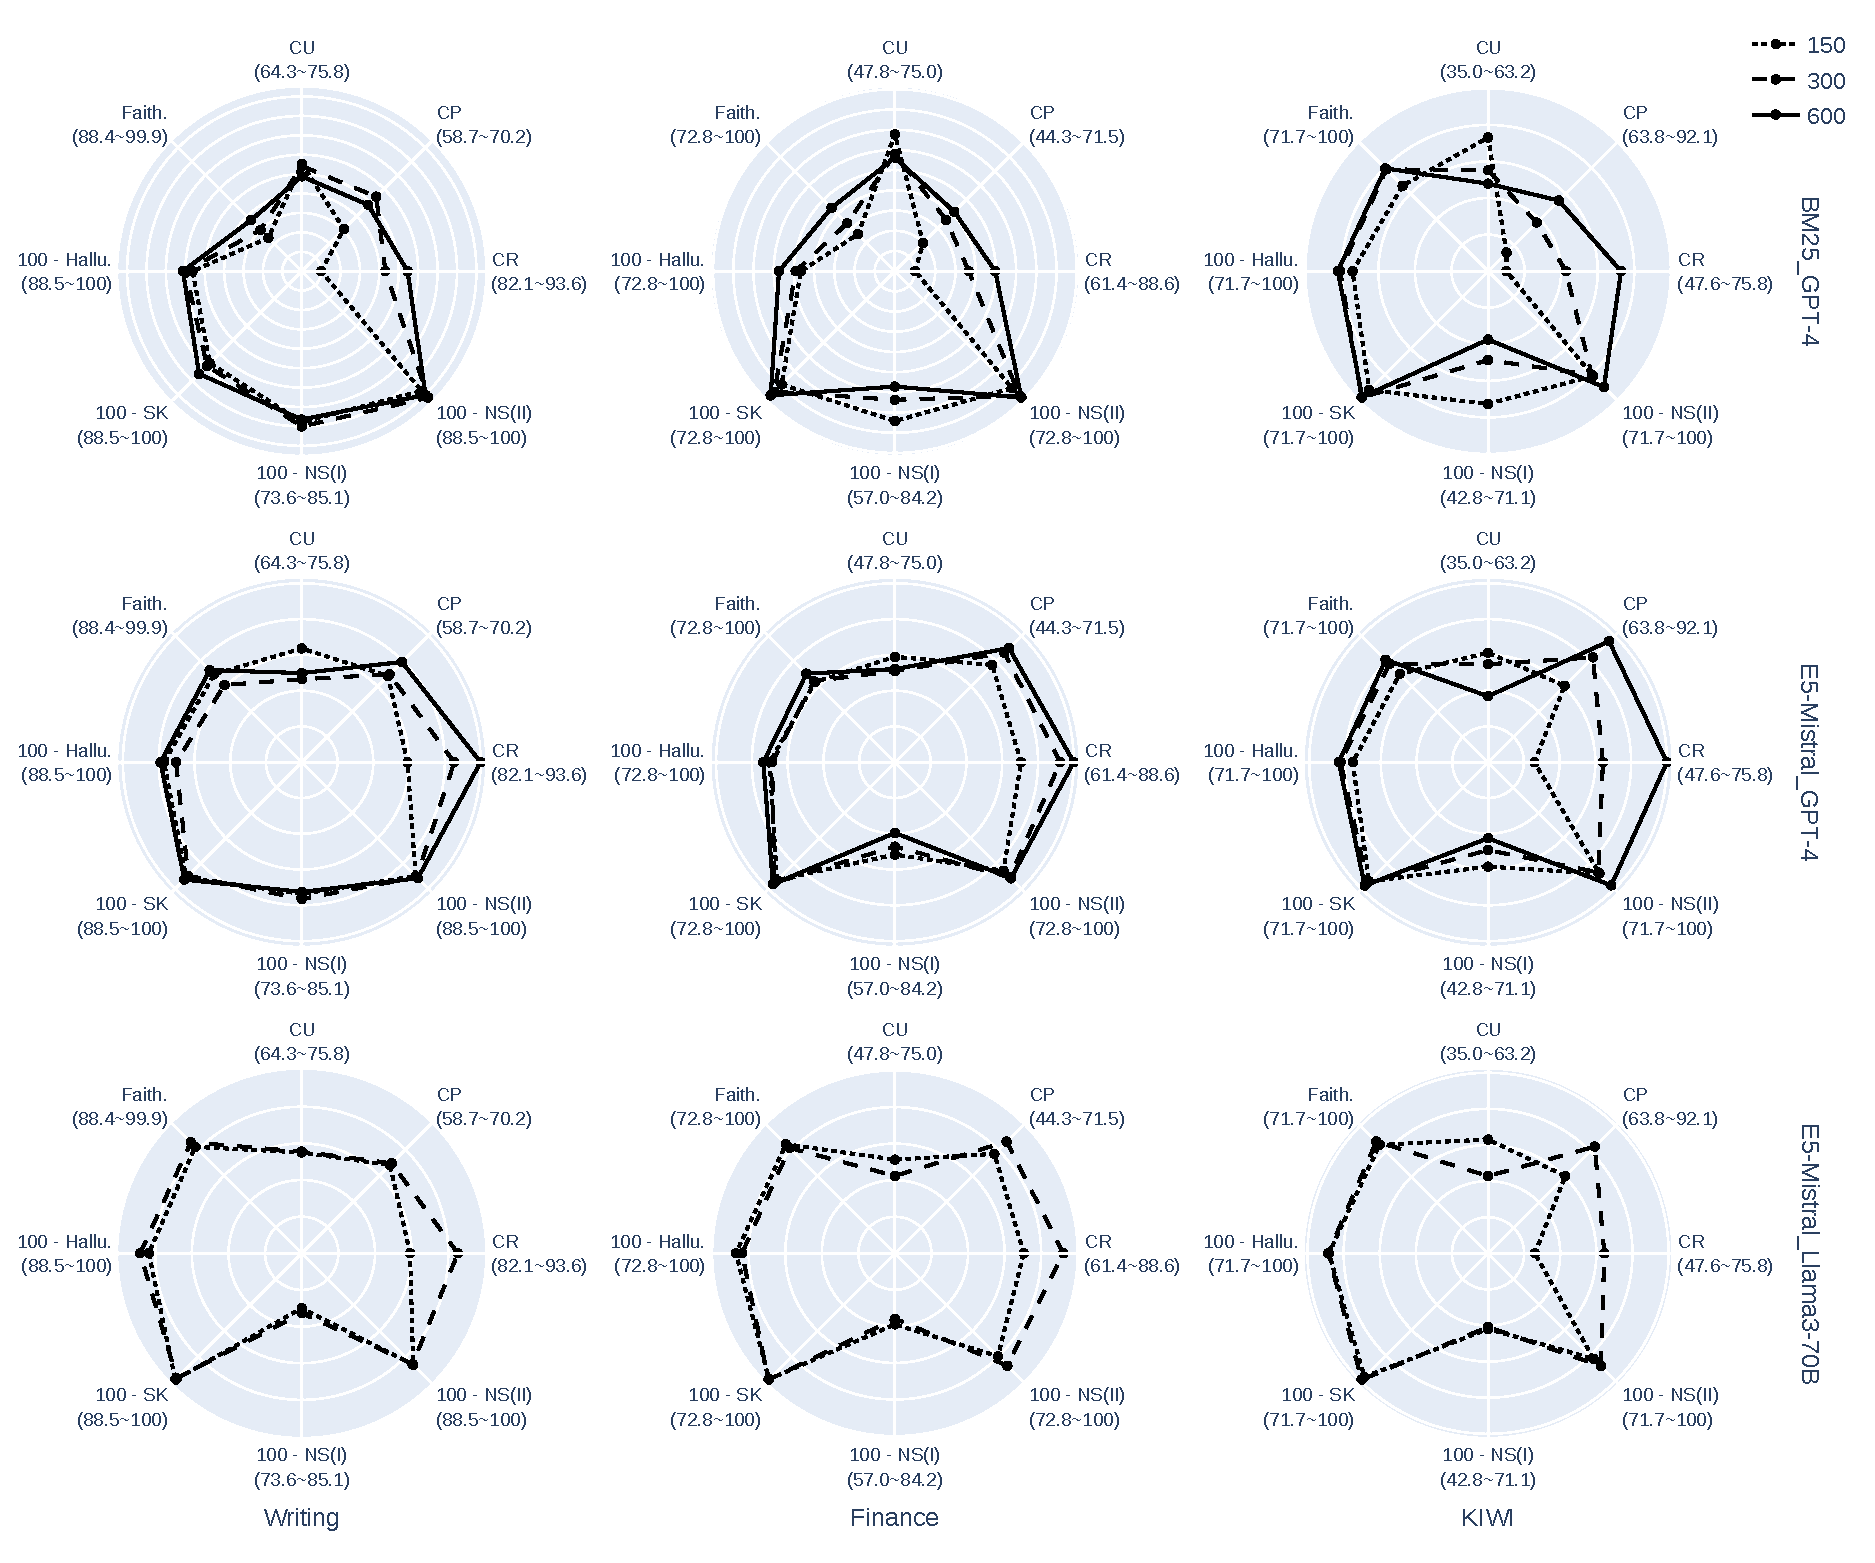
\includegraphics[width=\columnwidth]{figures/radar_chunk_size.pdf}
    \caption{Diagnosis on Chunk Size}
    \label{fig:radar-chunk-size}
\end{figure}

\paragraph{More Context Enhances Faithfulness}
Top-k selection and chunk size both balance the amount of noise and useful information presented to the generator, but in different manners. Corresponding results are demonstrated in Fig.~\ref{fig:radar-topk} and Fig.~\ref{fig:radar-chunk-size}. Increasing $k$ adds more context that could be less relevant, while increasing chunk size provides more surrounding context of relevant facts. Thus \emph{context precision} decreases with larger $k$ but increases with larger chunk sizes. Despite this, they both lead to better \emph{claim recall} in Retrieval.

Generators tend to be more faithful when provided with more context, though this trend is less pronounced for Llama3, which already exhibits high faithfulness. \emph{Context utilization} generally worsens with more context due to increasing noise, leading to higher \emph{relevant noise sensitivity}.

Overall, the end-to-end RAG performance is slightly better with more context, primarily due to improved \emph{recall}. We recommend moderately increasing the two parameters for more faithful generation, noting that saturation occurs at high values as the amount of useful information is limited. Given a limited context length, a larger chunk size with a smaller k is preferred, especially for easier datasets (Finance, Writing). This is evident when comparing a chunk size of 150 with $k$=20 against a chunk size of 300 with $k$=10.

% \paragraph{Top-k Selection}  The number of chunks selected as context for generation balances the amount of noise and useful information presented to the generator. We compare using  $k \in\{5,10\}$ against our default setting of 20, which is already quite large.

% As shown in Fig.~\ref{fig:radar-topk}, Claim Recall increases while Context Precision decreases as more chunks are involved, regardless of whether sparse or dense retrieval is used. For the GPT-4 generator, it tends to be more faithful to the provided context with more chunks, whereas the trend is less pronounced for Llama3, which already has high faithfulness. Context Utilization generally worsens with larger k because the inclusion of more noisy chunks disrupts generation, leading to higher Noise Sensitivity in Relevant contexts. However, Noise Sensitivity in Irrelevant contexts slightly decreases as more relevant chunks become available as knowledge sources. As a combined effect of these nuanced aspects, the end-to-end RAG system typically achieves slightly better or comparable precision and improved recall, resulting in a slightly better overall F1 score.

% Based on these observations, we recommend involving more chunks as context for generation, especially for harder tasks like scientific reading (KIWI). Note that the benefits of increasing k saturate earlier on easier datasets (Finance and Writing), which require less context to answer.



% \paragraph{Chunk Size}  We compare chunk sizes of 100 and 600 against our default setting of 300. Due to the limited 8K context window of Llama3, we omit the experiment of chunk size 600 for the combination E5-Mistral+Llama3-70B.

% Larger chunk sizes lead to easier retrieval, with each chunk having a higher probability of including useful information and more text overall to help answer the query. However, generation becomes more difficult with longer context to process, increasing the challenge of identifying useful parts within the context.

% As shown in Fig.~\ref{fig:radar-chunk-size}, retrieval performance generally improves for both Claim Recall and Context Precision with larger chunk sizes. The trend levels off for sizes greater than 300 in Finance and Writing, as documents in these datasets are generally shorter (only 13\% longer than 300 tokens in Writing and 16\% in Finance). For other metrics on generators and overall performance, we observed a similar trend and saturation effect as seen in Top-k Selection, as both approaches provide more context to the generator. Therefore, moderately increasing chunk size can help improve final generation performance. Given a limited context window, a larger chunk size with a smaller k is preferred, especially for easier datasets (Finance, Writing). This is evident when comparing a chunk size of 150 with k=20 against a chunk size of 300 with k=10.

\begin{figure}[ht]
    \centering
    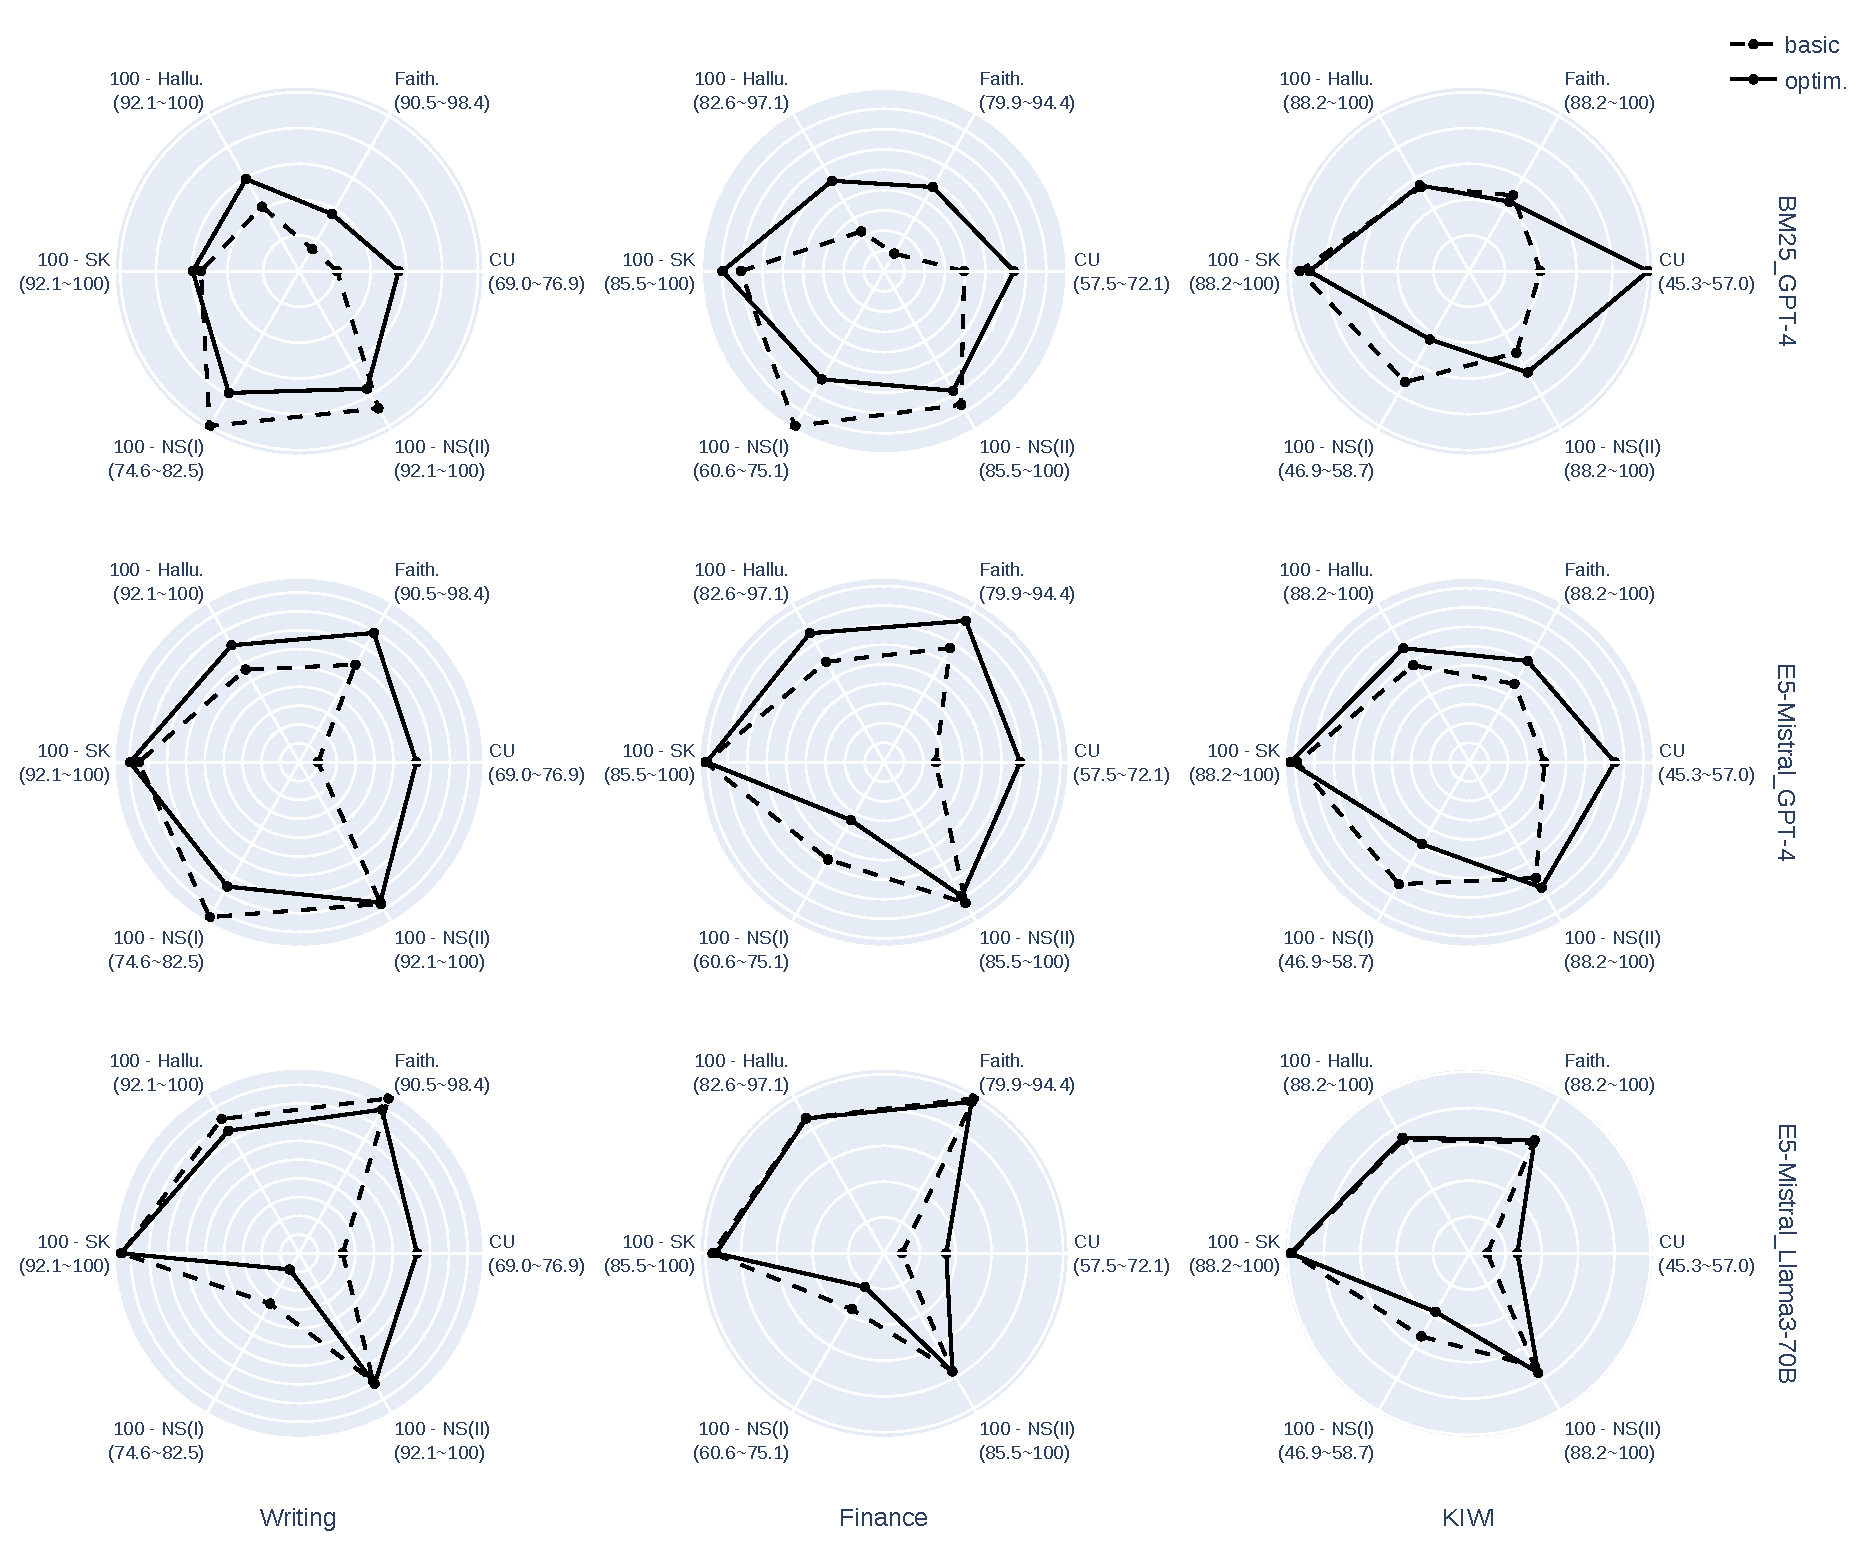
\includegraphics[width=\columnwidth]{figures/radar_prompt.pdf}
    \caption{Diagnosis on Generation Prompts}
    \label{fig:radar-prompt}
\end{figure}

\paragraph{Explicit Requirements in Prompts Affect Generation Preferences}  To validate the effect of the generation prompt, we added more detailed requirements to guide the generation for better \emph{faithfulness}, \emph{context utilization}, and lower \emph{noise sensitivity}. The optimized prompt is shown in Fig.~\ref{fig:improved_generation_prompt}.

\begin{figure}
    \centering
    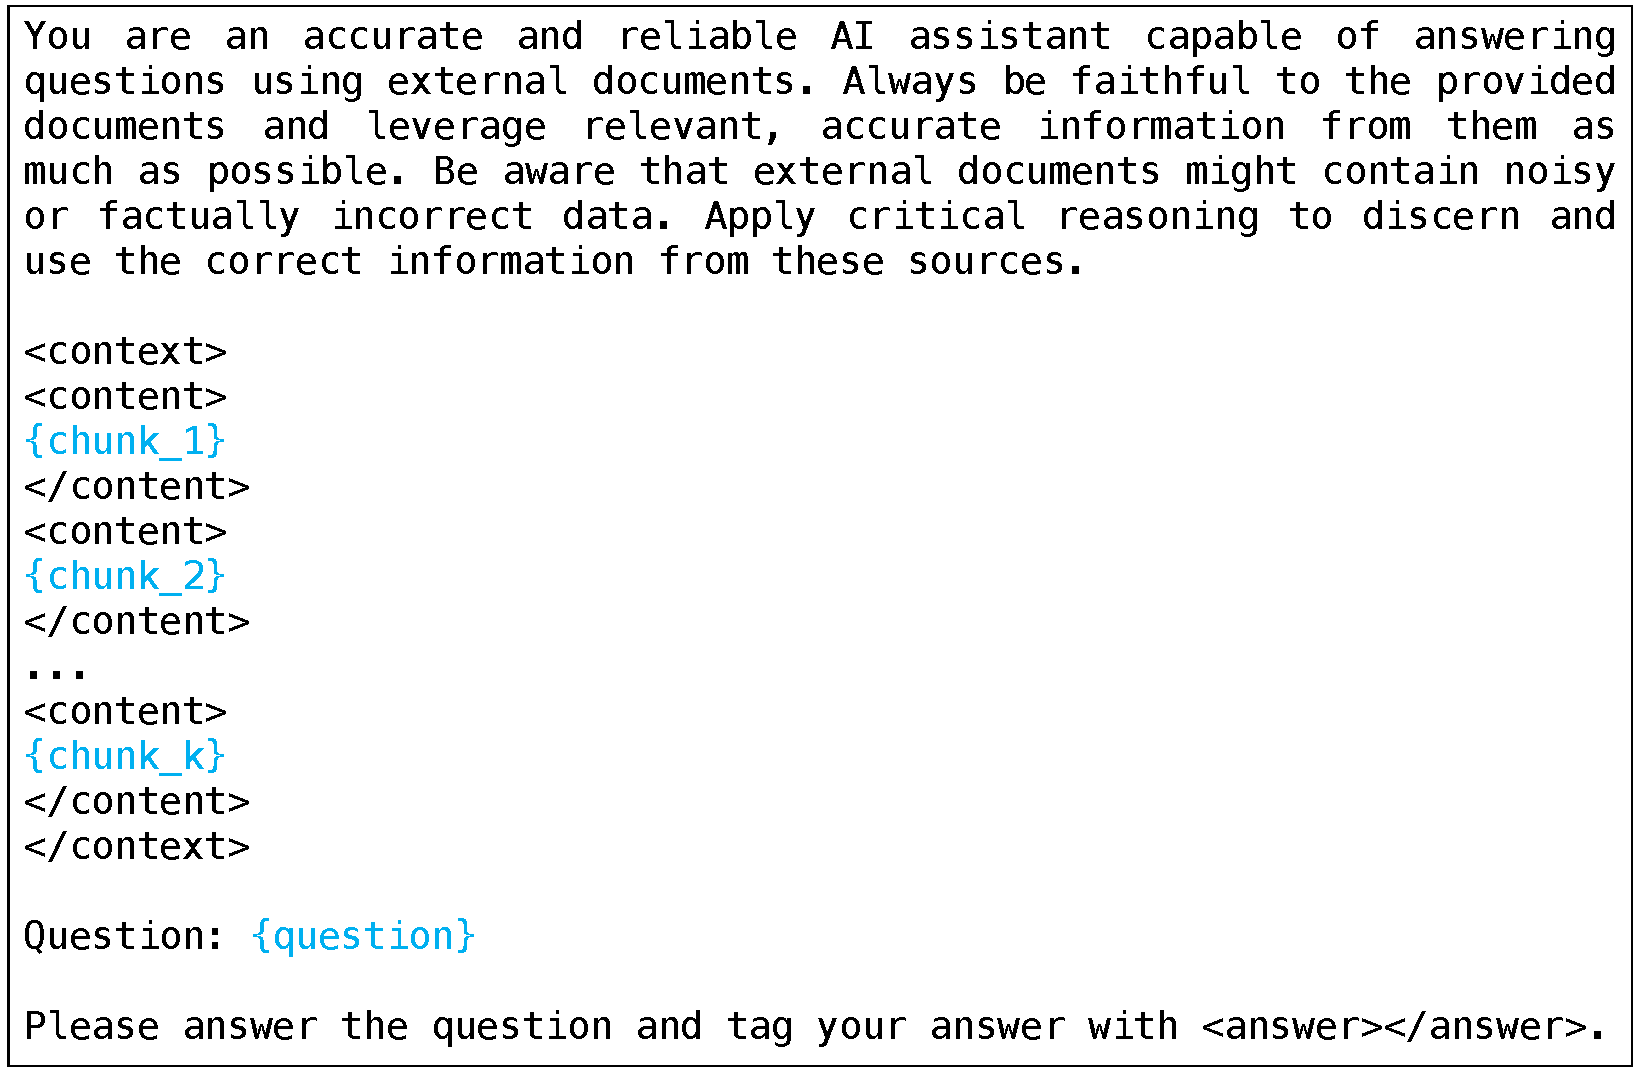
\includegraphics[width=0.8\textwidth]{figures/improved_generation_prompt.pdf}
    \caption{The optimized prompt for response generation. In this prompt, we explicitly instruct the LLMs to be faithful to the context and identify relevant information as possible.}
    \label{fig:improved_generation_prompt}
\end{figure}

As shown in Fig.~\ref{fig:radar-prompt}, we observed a general improvement in \emph{context utilization}. However, as a counterpart to \emph{context utilization}, \emph{noise sensitivity} generally worsened. It demonstrates the difficulty of meeting all prompt requirements when there are subtle tension between them.

For the two generators, GPT-4 generally showes improvements in metrics related to faithfulness (\emph{hallucination}, \emph{self-knowledge}, \emph{faithfulness}), whereas Llama3 does not exhibit the same behavior. This aligns with our previous observation (Sec.~\ref{sec:analysis}) that Llama3 already performs well on \emph{faithfulness}, while GPT-4 tends to rely on self-knowledge without explicit requirements. Consequently, there is a steady improvement in overall \emph{F1} for GPT-4 when switched to the optimized prompt, while the difference for Llama3 is negligible.

RAG builders can optimize prompts by combining performance on modular metrics provided by \benchname\space with user preferences and generator capabilities on different aspects.

\begin{figure}[ht]
    \centering
    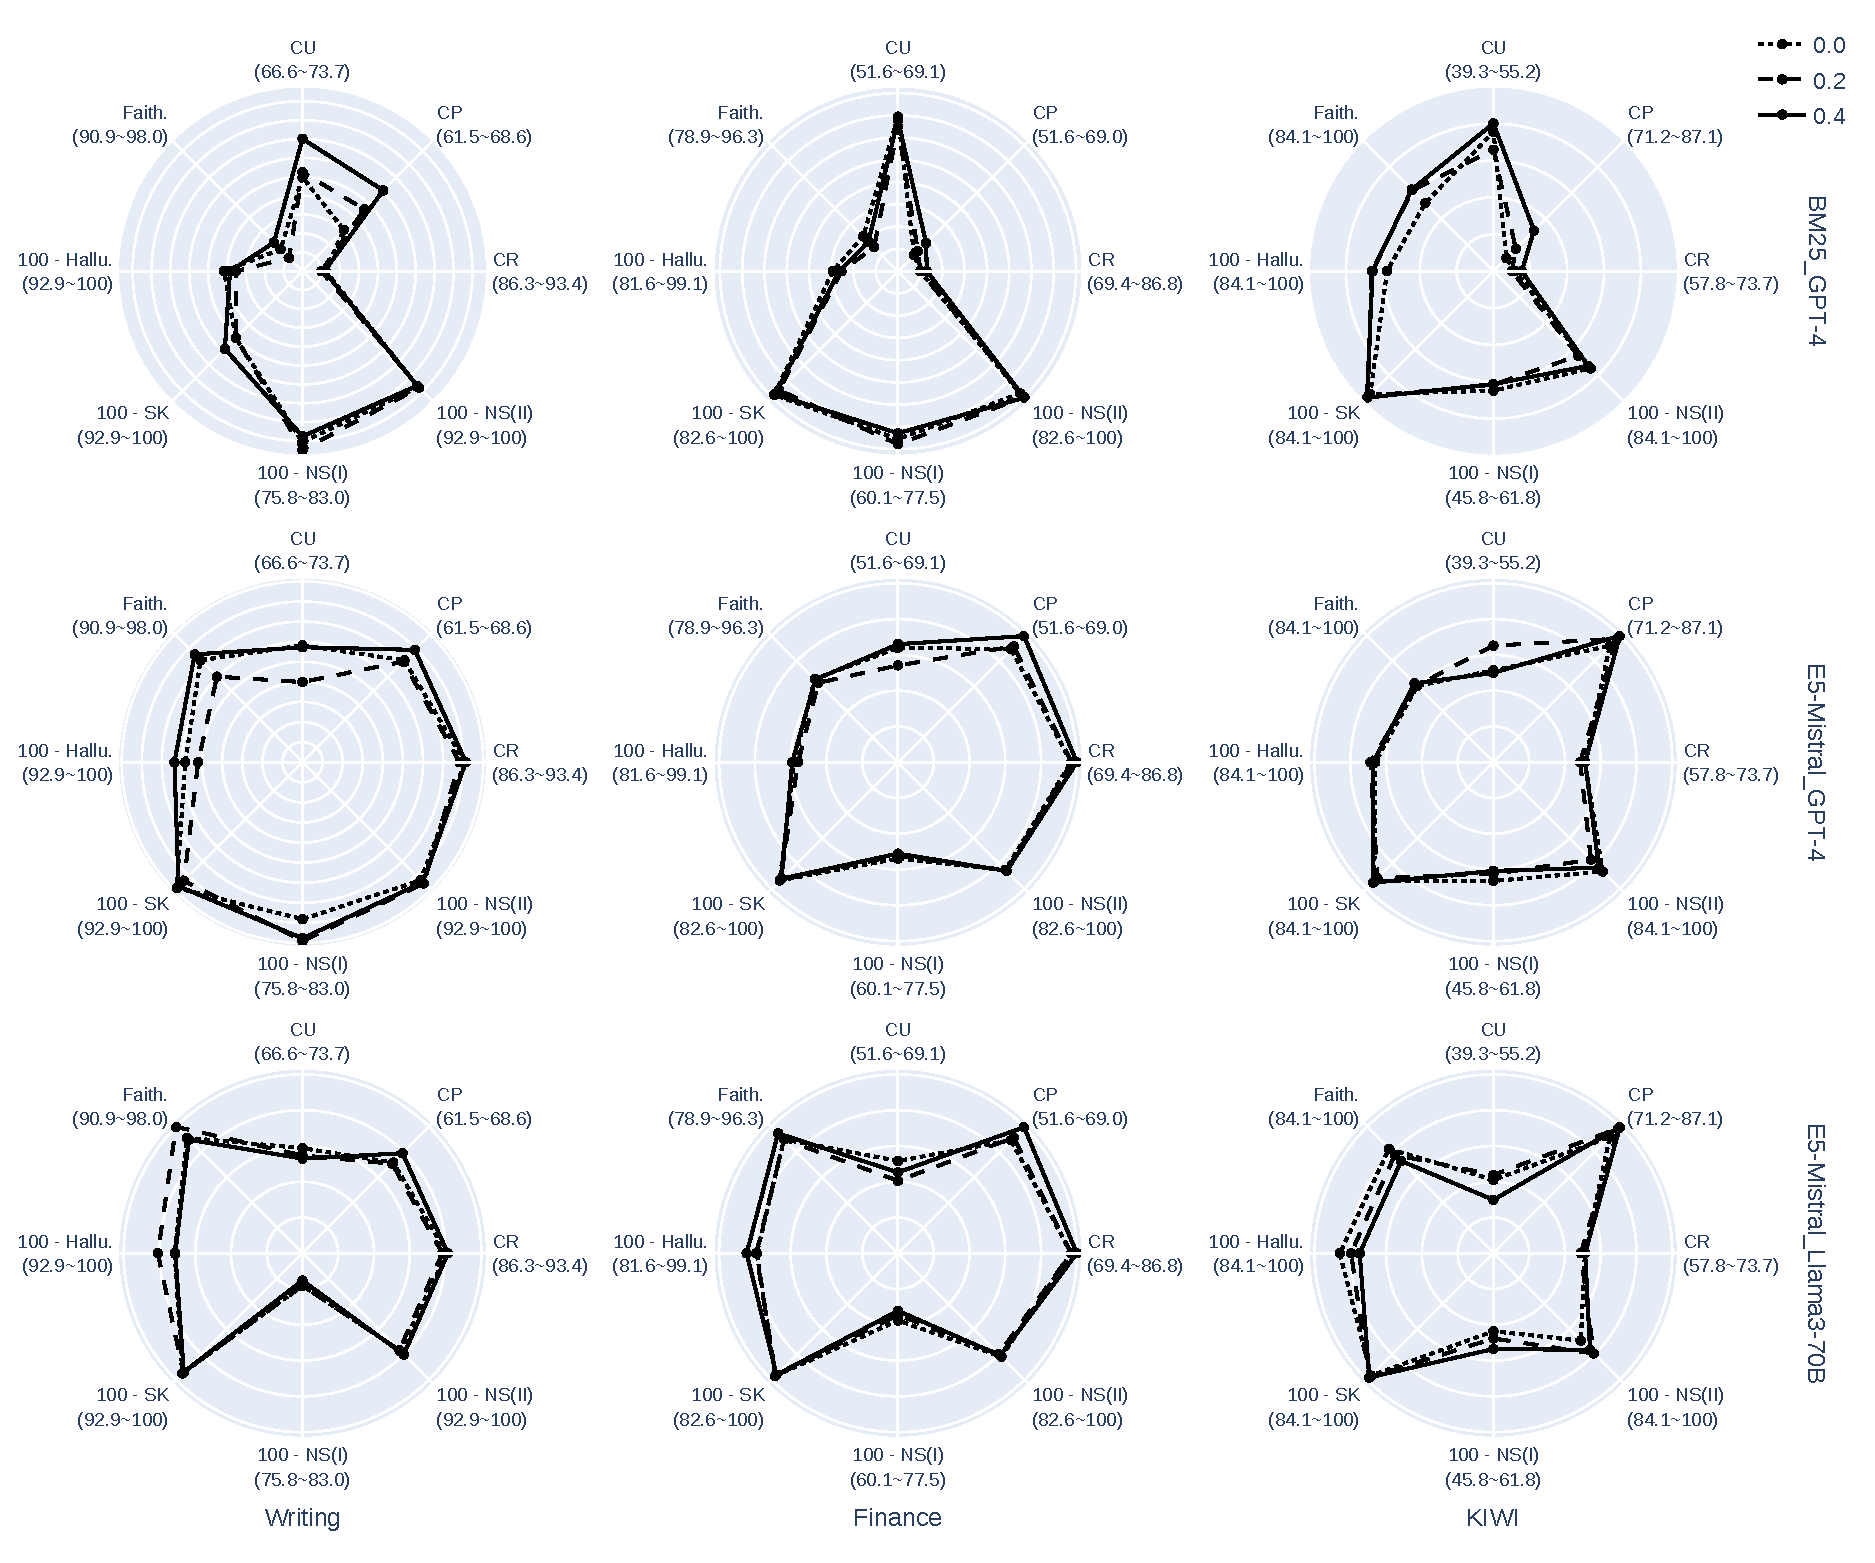
\includegraphics[width=\columnwidth]{figures/radar_overlap_ratio.pdf}
    \caption{Diagnosis on Chunk Overlap Ratio}
    \label{fig:radar-overlap-ratio}
\end{figure}

\paragraph{Chunk Overlap Does Not Matter a Lot}  Chunk overlap ratio between adjacent chunks is usually set to be non-zero to help the generator better utilize surrounding information and identify chunks with coherent logic, thus alleviating the impact of hard splits in significant semantics.

According to our results in Fig.~\ref{fig:radar-overlap-ratio}, higher overlap ratios generally lead to improved \emph{context precision}. However, this does not necessarily translate to an increase in the total amount of useful information retrieved. This phenomenon can be attributed to the retrieval of more chunks that contain the same segment of useful information. Consequently, we observed that overlap ratio adjustments do not have a significant impact on other performance metrics in a consistent and obvious manner. This suggests that the overlap ratio may not require extensive tuning in practice.